\documentclass[12pt]{article}
\usepackage{mathtools}
\usepackage{amssymb}
\usepackage{amsthm}
\usepackage{pgfplots}
\usepackage{tikz}
\usetikzlibrary{calc}
\usepackage{polski}
\usepackage[utf8]{inputenc}
\usepackage{geometry}
\usepackage{amsmath}
\usepackage{gensymb}
\usepackage{mnsymbol}
\usepackage{graphicx}
\usepackage{textgreek}
\usepackage{float}
\usepackage{caption}
\begin{document}
\newgeometry{tmargin=2cm,bmargin=2cm,lmargin=2cm,rmargin=2cm}
\tableofcontents \newpage
\section{Cel ćwiczenia}
Celem ćwiczenia było zapoznanie się z budową i działaniem przyrządu zwanego busolą stycznych oraz wyznaczenie składowej poziomej ziemskiego pola magnetycznego.
\section{Wstęp teorytyczny}
\textbf{Indukcja magnetyczna} jest to fizyczna wartość wektorowa definiująca pole magnetyczne. Wyznacza się ją za pomocą siły Lorentza działającej na naładowany obiekt poruszający się polu magnetycznym. Do wyznaczania indukcji magnetycznej służy wzór: 
\begin{center}
\Large $\vec{F}=q(\vec{v}\times\vec{B}) $,
\end{center}
gdzie $\vec{B}$ to wektor indukcji magnetycznej, $\vec{F}$ to wektor siły Lorentza, $q$ to ładunek elektryczny , a $\vec{v}$ to wektor prędkości obiektu naładowanego elektrycznie poruszającego się w polu elektrycznym. \newline
\textbf{Prawo Biota-Savarta} służy do wyznaczania wartości indukcji pola magnetycznego $dB$ w określonym punkcie, powodowanej przez bardzo mały odcinek przewodnika $dl$, przez który przepływa prąd o natężeniu I. Można je zapisać w postaci wzoru: 
\begin{center}
\Large $ d\vec{B}=\frac{\mu_0\vec{I}}{4\pi}\frac{d\vec{l}{\times}\vec{r}}{r^3}$,
\end{center}
gdzie $d\vec{B}$ to wektor indukcji magnetycznej powodowanej przez bardzo mały odcinek przewodnika $d\vec{l}$, $\mu_0$ to przenikalność magnetyczna próżni ($\mu_0=4\pi*10^{-7}\frac{Vs}{Am})$, $\vec{I}$ to wektor natężenia prądu elektrycznego, $d\vec{l}$ to wektor nieskończenie krótkiego odcinka przewodnika elektrycznego zaś $\vec{r}$ to wektor odległości wychodzącej od bardzo małego przewodnika elektrycznego do punktu, w którym wyznaczana jest wartość indukcji magnetycznej. \newline
Do obliczenia indukcji magnetycznej działającej na punkt będący w środku koła, którym jest przewodnik z prądem, możemy wykorzystać prawo Biota-Savarta. Dla środka cewki kołowej, lub bardzo krótkiej zwojnicy złożonej z $N$ zwojów wartość indukcji pola magnetycznego wynosi : 
\begin{center}
\Large $ B = \mu_0\frac{NI}{2r}$,
\end{center}
Wiedza na temat wartości indukcji pola magnetycznego w środku cewki kołowej pozwala zbudować przyrząd do pomiaru składowej poziomej pola magnetycznego Ziemi, zwany busolą stycznych. W przyrządzie tym wykorzystano oddziaływanie pola magnetycznego wytworzonego przez cewkę z prądem, z igłą magnetyczną. Na cienką obręcz wykonaną z materiału nieferromagnetycznego
(np. mosiądz lub aluminium) nawinięto uzwojenia cewki, najczęściej wykonane z miedzi. W środku obręczy znajduje się igła magnetyczna przytwierdzona w taki sposób, by mogła się obracać swobodnie w płaszczyźnie poziomej. Gdy w cewce nie płynie prąd igła magnetyczna ustawia się równolegle do składowej poziomej pola ziemskiego $B_0$. Busolę można tak ustawić, by kierunek wektora $B_0$ znajdował się w płaszczyźnie zwojów. Oddziaływanie pola z momentem magnetycznym igły sprawia, że igła ustawia się zgodnie z wektorem poziomej składowej pola wypadkowego. Po włączeniu prądu powstaje pole $B$ o kierunku prostopadłym do płaszczyzny zwojów, co indukuje ustawienie igły magnetycznej w kierunku wypadkowej obu pól. Wektory $\vec{B}$,$\vec{B_0}$ oraz
$\vec{B_w}$ tworzą trójkąt prostokątny (rysunek na kolejnej stronie), z którego widać zależność:
\begin{center}
\Large $\frac{B}{B_0}=tg\alpha \;\;\; => \;\;\; B_0=\frac{B}{tg\alpha}=\mu_0\frac{NI}{2Rtg\alpha}$
\end{center}
\begin{figure}[H]
\centering
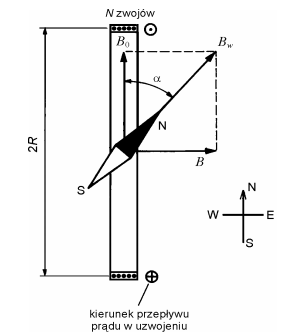
\includegraphics[width=8cm]{Dodatek1}
\end{figure} 
Jednostką indukcji magnetycznej jest tesla [T]. Wartość jednej tesli jest równa sile (Lorentza) jaka działa na ładunek 1C poruszający się z prędkością 1 metra na sekundę.
\begin{center}
\Large $ [T] = [\frac{N}{Am}]$,
\end{center}
Natężenie pola magnetycznego to wielkość wektorowa, odpowiadająca sile działającej na jednostkowy ładunek elektryczny poruszający się z jednostkową prędkością w kierunku prostopadłym do tej wielkości wektorowej. Jednostką natężenia pola magnetycznego jest amper na metr ($[\frac{A}{m}]$) \newline
Amper to jednostka natężenia prądu elektrycznego. Jest jednostką podstawową w układzie SI. Jeśli przepływający przez dany przekrój prąd ma natężenie $1A$, oznacza to, że w ciągu $1s$ przepływa $1C$ ładunku, czyli: 
\begin{center}
\Large $ 1A = \frac{1C}{1s}$,
\end{center}
Biegun magnetyczny to miejsce igły magnetycznej, magnesu trwałego lub elektromagnesu, w którym natężenie pola magnetycznego ma największą wartość. Pola magnesu sztabkowego i pole magnetyczne Ziemi:
\begin{figure}[H]
\centering
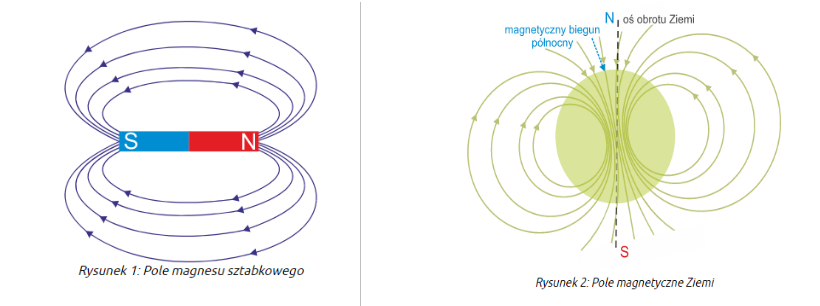
\includegraphics[width=15cm]{Konspekt1}
\end{figure} 
\section{Układ pomiarowy}
Przyrządy potrzebne do wykonania doświadczenia (Rys. 4): \newline
1. Busola stycznych \newline 
2. Zasilacz napięcia stałego \newline
3. Amperomierz \newline
4. Opornica suwakowa \newline 
5. Przełącznik kierunku prądu \newline
6. Kalkulator \newline
\begin{figure}[H]
\centering
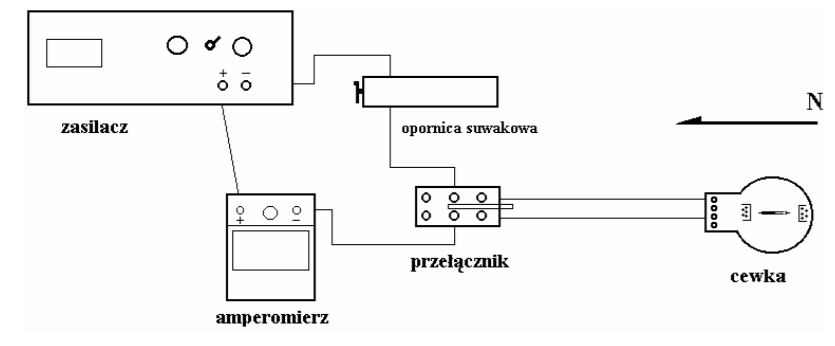
\includegraphics[width=11cm]{4}
\caption*{\textbf{Rys. 1}: Układ elektryczny busoli stycznych}
\end{figure} \newpage
\section{Przebieg ćwiczenia}
Doświadczenie zaczęliśmy od zapoznania się z elementami układu pomiarowego, odsunięcia busoli stycznych maksymalnie od zasilacza oraz wypoziomowania 
podstawy busoli. Po ustawieniu płaszczyzny zwojów w płaszczyźnie południka magnetycznego ziemskiego oraz konsultacji z prowadzącym zajęcia przygotowaliśmy się do pomiarów. Następnie dla różnej ilości zwojów $N$ oraz różnego natężenia prądu $I$ odczytywaliśmy kąt wychylenia igły $\alpha$ dla obu kierunków przepływu prądu. Wyniki zestawiliśmy w tabeli.
\section{Wyniki pomiarów}
\begin{figure}[H]
\centering
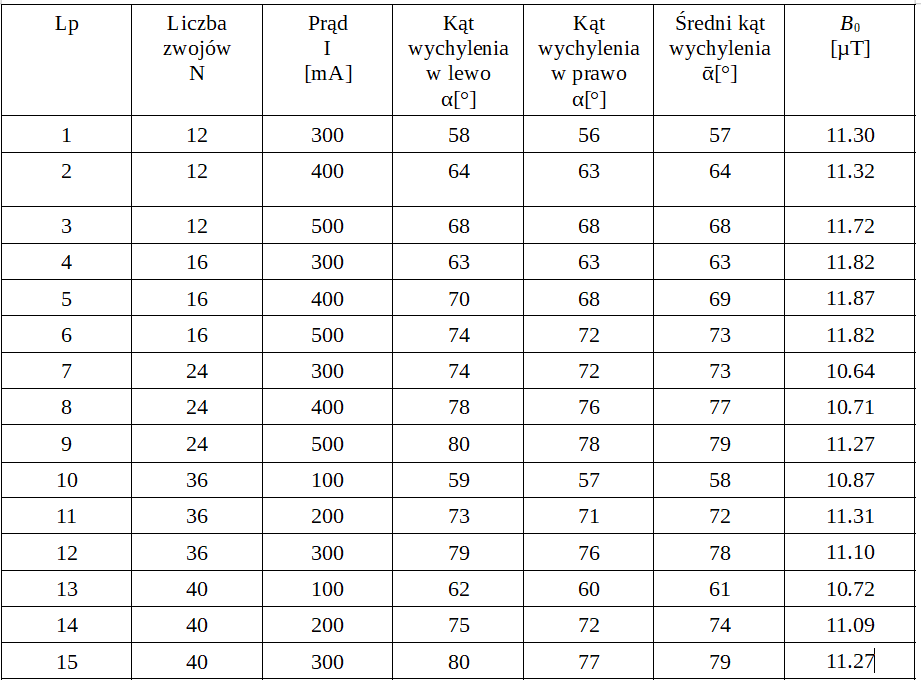
\includegraphics[width=15cm]{5}
\caption*{\textbf{Tab. 1}: Tabela z wynikami pomiarów}
\end{figure} 

Klasa amperomierza - $0.5$ \newline
Średnica cewki - $260\;mm$ \newline
Niepewność pomiaru średnicy cewki - $3\;mm$
\section{Opracowanie wyników pomiarów}
\subsection{Wartość składowej poziomej indukcji ziemskiego pola magnetycznego każdego z pomiarów}
Korzystając z wyników pierwszego pomiaru oraz wzoru:
\begin{center}
\Large $B_0=\mu_0\frac{NI}{2Rtg\alpha} = 4\pi*10^{-7}\frac{Vs}{Am}\frac{12*300mA}{0.26m*tg(57\degree)} = 11.30\mu{T}$
\end{center}
Dla reszty pomiarów wykonaliśmy analogiczne obliczenia.
\subsection{Średni wynik wartości składowej poziomej indukcji ziemskiego pola magnetycznego}
Jako średni wynik wartości składowej poziomej indukcji ziemskiego pola magnetycznego przyjęliśmy średnią arytmetyczną z wszystkich wartości $B_0$ obliczonych oraz wpisanych do tabeli dla każdego z pomiarów:
\begin{center}
\Large $\bar{B} = 11.26\;\mu{T}$
\end{center}
\subsection{Obliczanie niepewności pomiaru składowej poziomej indukcji ziemskiego pola magnetycznego}
Obliczając wartość składowej poziomej indukcji ziemskiego pola magnetycznego posługujemy się wzorem:
\begin{center}
\Large $B_0=\mu_0\frac{NI}{2Rtg\alpha}. $
\end{center}
(a) Błąd przypadkowy \newline
W związku z tym, że wartości $\mu_0$ oraz $N$ znamy bezbłędnie, głównym źródłem błędu przypadkowego jest pomiar kąta $\alpha$. 
Miarą tego błędu jest niepewność pomiaru typu $A$:
\begin{center}
\Large $u_A(B_0) = \sqrt{\frac{\sum_{n=1}^{15} (B_i-\bar{B})^2}{15*14}}\;\mu{T} = 0.11\;\mu{T}$
\end{center}
Zaś niepewność względna:
\begin{center}
\Large $\frac{u_A(B_0)}{B_0}*100\% = 0.98\%$
\end{center}
(b) Błąd systematyczny $1$ \newline
Pierwszym źródłem błędu systematycznego jest amperomierz. Jego niepewność graniczna możemy obliczyć przy pomocy jego klasy dokładności wynosi:
\begin{center}
\Large $\Delta{I} = \frac{zakres*{klasa}}{100} = \frac{0.5*750\;mA}{100} = 3.8\;mA $
\end{center}
Jego niepewność standardowa wynosi:
\begin{center}
\Large $u_B(I) = \frac{\Delta{I}}{\sqrt{3}} = \frac{3.8\;mA}{\sqrt{3}}=2.2\;mA $
\end{center}
Zatem jego niepewność względna:
 \begin{center}
\Large $\frac{u_B(I)}{I} = \frac{2.2\;mA}{375\;mA}*100\% = 0.58\% $
\end{center}
(c) Błąd systematyczny $2$ \newline
Drugim źródłem błędu systematycznego jest błąd pomiaru promienia. Przyjmując $u_B(R)=3\;mm$ otrzymujemy niepewność względną:
\begin{center}
\Large $ \frac{u_B(R)}{R} = \frac{3\;mm}{260\;mm}*100\% =1.2\%$ 
\end{center}
(d) Niepewność złożona $u_C(B_0)$ \newline
Używając powyższych wyników jesteśmy w stanie obliczyć względną niepewność złożoną $u_C(B_0)$:
\begin{center}
\Large $ \frac{u_C(B_0)}{B_0}=\sqrt{(\frac{u_A(B_0)}{B_0})^2+(\frac{u_B(I)}{I}^2)+(\frac{u_B(R)}{R})^2} = \sqrt{(0.0098)^2+(0.0058)^2+(0.012)^2} = 0.017 = 1.7\%$
\end{center} 
Stąd niepewność złożona $u_C(B_0)$:
\begin{center}
\Large $ u_C(B_0) = B_0*\sqrt{(\frac{u_A(B_0)}{B_0})^2+(\frac{u_B(I)}{I}^2)+(\frac{u_B(R)}{R})^2} = 0.017*1.225\;\mu{T} = 0.19\;\mu{T}$ 
\end{center}
Zaś niepewność rozszerzona $U_C(B_0)$:
\begin{center}
\Large $ U_C(B_0) = k*u_C(B_0) = 0.38\;\mu{T}$ 
\end{center}
\section{Wnioski}
Zmierzona wartość składowej poziomej indukcji ziemskiego pola magnetycznego wynosi $B_0 = 11.26\;\mu{T}$, zaś jej niepewność rozszerzona $U_C(B_0) = 0.38\;\mu{T}$. Wartość tabelaryczna, jak podaje opis ćwiczenia, to $21\;\mu{T}$. Otrzymany wynik znacznie róźni się od wartości tabelarycznej, nawet po uwzględnieniu niepewności rozszerzonej. Najprawdopobniej przyczyną tej niezgodności były błędy przypadkowe i systematyczne takie jak zły pomiar kąta $\alpha$, niedokładność amperomierza, zły pomiar promieniu, a także źle wypoziomowa lub odwrócona busola stycznych. Możliwą przyczyną była również obecność urządzeń elektronicznych w pobliżu busoli, zakłócających pole magnetyczne oraz wskazania igły magnetycznej. 
\end{document}
